%\setchapterimage{fig_00.jpg}
\chapter*{Application \arabic{cptApplication} \\ 
Machines Synchrones -- Alternateur et Moteur
-- \ifprof Corrigé \else Sujet \fi}
\addcontentsline{toc}{section}{Application \arabic{cptApplication} : 
Machines Synchrones -- Alternateur et Moteur
-- \ifprof Corrigé \else Sujet \fi}

\iflivret \stepcounter{cptApplication} \else
\ifprof  \stepcounter{cptApplication} \else \fi
\fi

\setcounter{question}{0}
\marginnote{Ressources de Philippe Dubois.}

La plaque signalétique d’une machine synchrone triphasée porte les indications suivantes : 
\SI{100}{kVA} ; 230/400 \si{V} ; \SI{50}{Hz} ; \SI{1000}{tr/min}. 

La machine est couplée en étoile.
Un essai à vide, en alternateur, à vitesse de synchronisme a montré que sa caractéristique $E=f(I_e)$   est une droite passant par l’origine et par le point $E = 200 V$ pour $I_e = \SI{20}{A}$.

Un essai en court-circuit à la vitesse de synchronisme montre que la caractéristique $\indice{I}{cc}=f(I_e)$ est aussi une droite passant par l’origine et par le point $\indice{I}{cc} = \SI{205}{A}$ pour $I_e = \SI{30}{A}$.
La résistance des enroulements statoriques est supposée négligeable. 

\subsection*{Etude en fonctionnement alternateur}

\question{Quel est le nombre de pôles de cette machine ?}
\ifprof
\begin{corrige}
On a $N_s = \dfrac{60f}{p}$ $\Rightarrow p = \dfrac{60f}{N_s}$ $=\dfrac{60\times 50}{1000}=3$ paires de pôles.

\end{corrige}
\else
\fi



\question{Déterminer la réactance synchrone ($L \omega$) d’un enroulement statorique de cette machine.\sidenote{On pourra utiliser l'essai en court-circuit.}
 %La machine fonctionne en alternateur.
 }
\ifprof
\begin{corrige}
On utilise le modèle suivant. 

\begin{center}
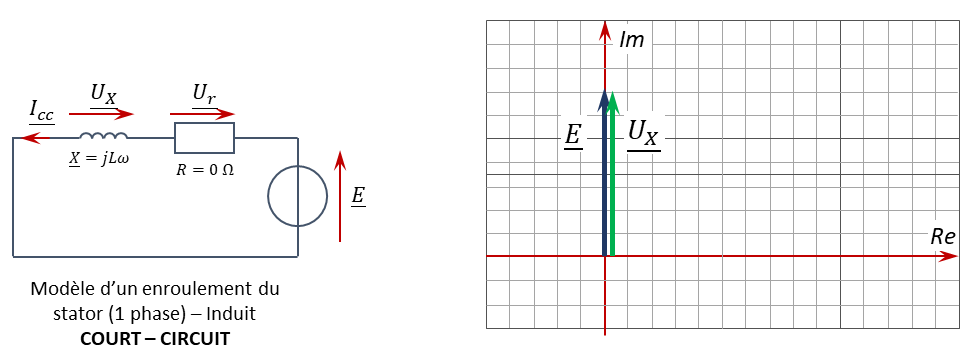
\includegraphics[width=\linewidth]{cor_01}
\end{center}

Pour le modèle en court-circuit, on a $\underline{I}=\indice{I}{cc}\sqrt{2}e^{j\left(\omega t\right)}$.

On a $E = 10 I_e $; donc pour \SI{30}{A}, $E_0=\SI{300}{V}$. En conséquences, $\underline{E}=E_0\sqrt{2}e^{j\left(\omega t + \varphi\right)}$.

$\underline{U_X}=\indice{I}{cc}jL\omega\sqrt{2}e^{j\left(\omega t\right)}$.


D'après la loi des mailles, $\underline{E} = \underline{U_X}$; donc 
$E_0\sqrt{2}e^{j\left(\omega t + \varphi\right)} = \indice{I}{cc}jL\omega\sqrt{2}e^{j\left(\omega t\right)}$ et $\varphi = \dfrac{\pi}{2}$.

Au final, $ L\omega =\dfrac{E_0}{\indice{I}{cc}} $.

\textit{AN :} $ L\omega =\dfrac{300}{205} = \SI{1,46}{\Omega}$.

\end{corrige}
\else
\fi

\question{Déterminer $I_e$ pour que la machine fournisse son intensité nominale, sous sa tension nominale, à une charge de facteur de puissance 0,93.}
\ifprof
\begin{marginfigure}
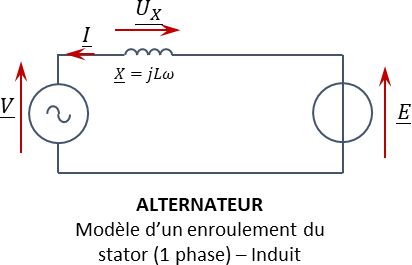
\includegraphics[width=\linewidth]{cor_02}
\end{marginfigure}

\begin{marginfigure}
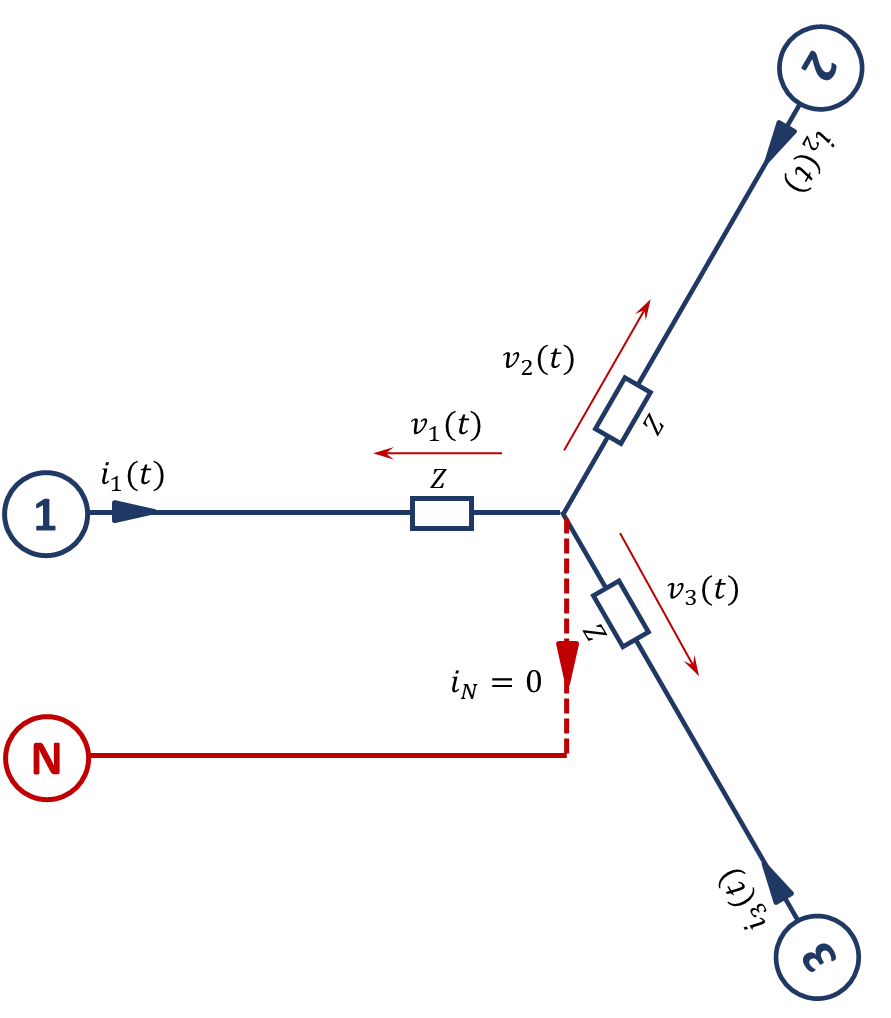
\includegraphics[width=\linewidth]{cor_03}
\end{marginfigure}

\begin{corrige}


\end{corrige}
\else
\fi

\subsection*{Etude en fonctionnement moteur}

La machine fonctionne en moteur, alimentée par un réseau triphasé 230/400\si{V}, \SI{50}{Hz}. Elle développe un couple de moment $C_u= \SI{610}{N.m}$.
Le rendement du moteur étant égal à 0,96 . 

\question{Déterminer la puissance active puis l’intensité efficace en ligne sachant que le facteur de puissance du moteur est égal à 1.}
\ifprof
\begin{corrige}


\end{corrige}
\else
\fi

\question{Quelle est alors la valeur de $I_e$ ?}
\ifprof
\begin{corrige}


\end{corrige}
\else
\fi

On règle $I_e$ à \SI{18,8}{A}. Sous la tension nominale, le moteur demande alors un courant en ligne d’intensité \SI{120}{A}. 

\question{Quel est le déphasage courant-tension ?}
\ifprof
\begin{corrige}


\end{corrige}
\else
\fi


\ifprof
\else
\begin{marginfigure}[-3cm]
\centering
%\includegraphics[width=3cm]{Cy_02_Ch_01_Activation_01_qr}
\end{marginfigure}
\fi




